\chapter{Projekt systemu Soccer Match Predictor}
\section{Ogólny schemat systemu i jego architektura}
    \begin{figure}[h] 
        \centering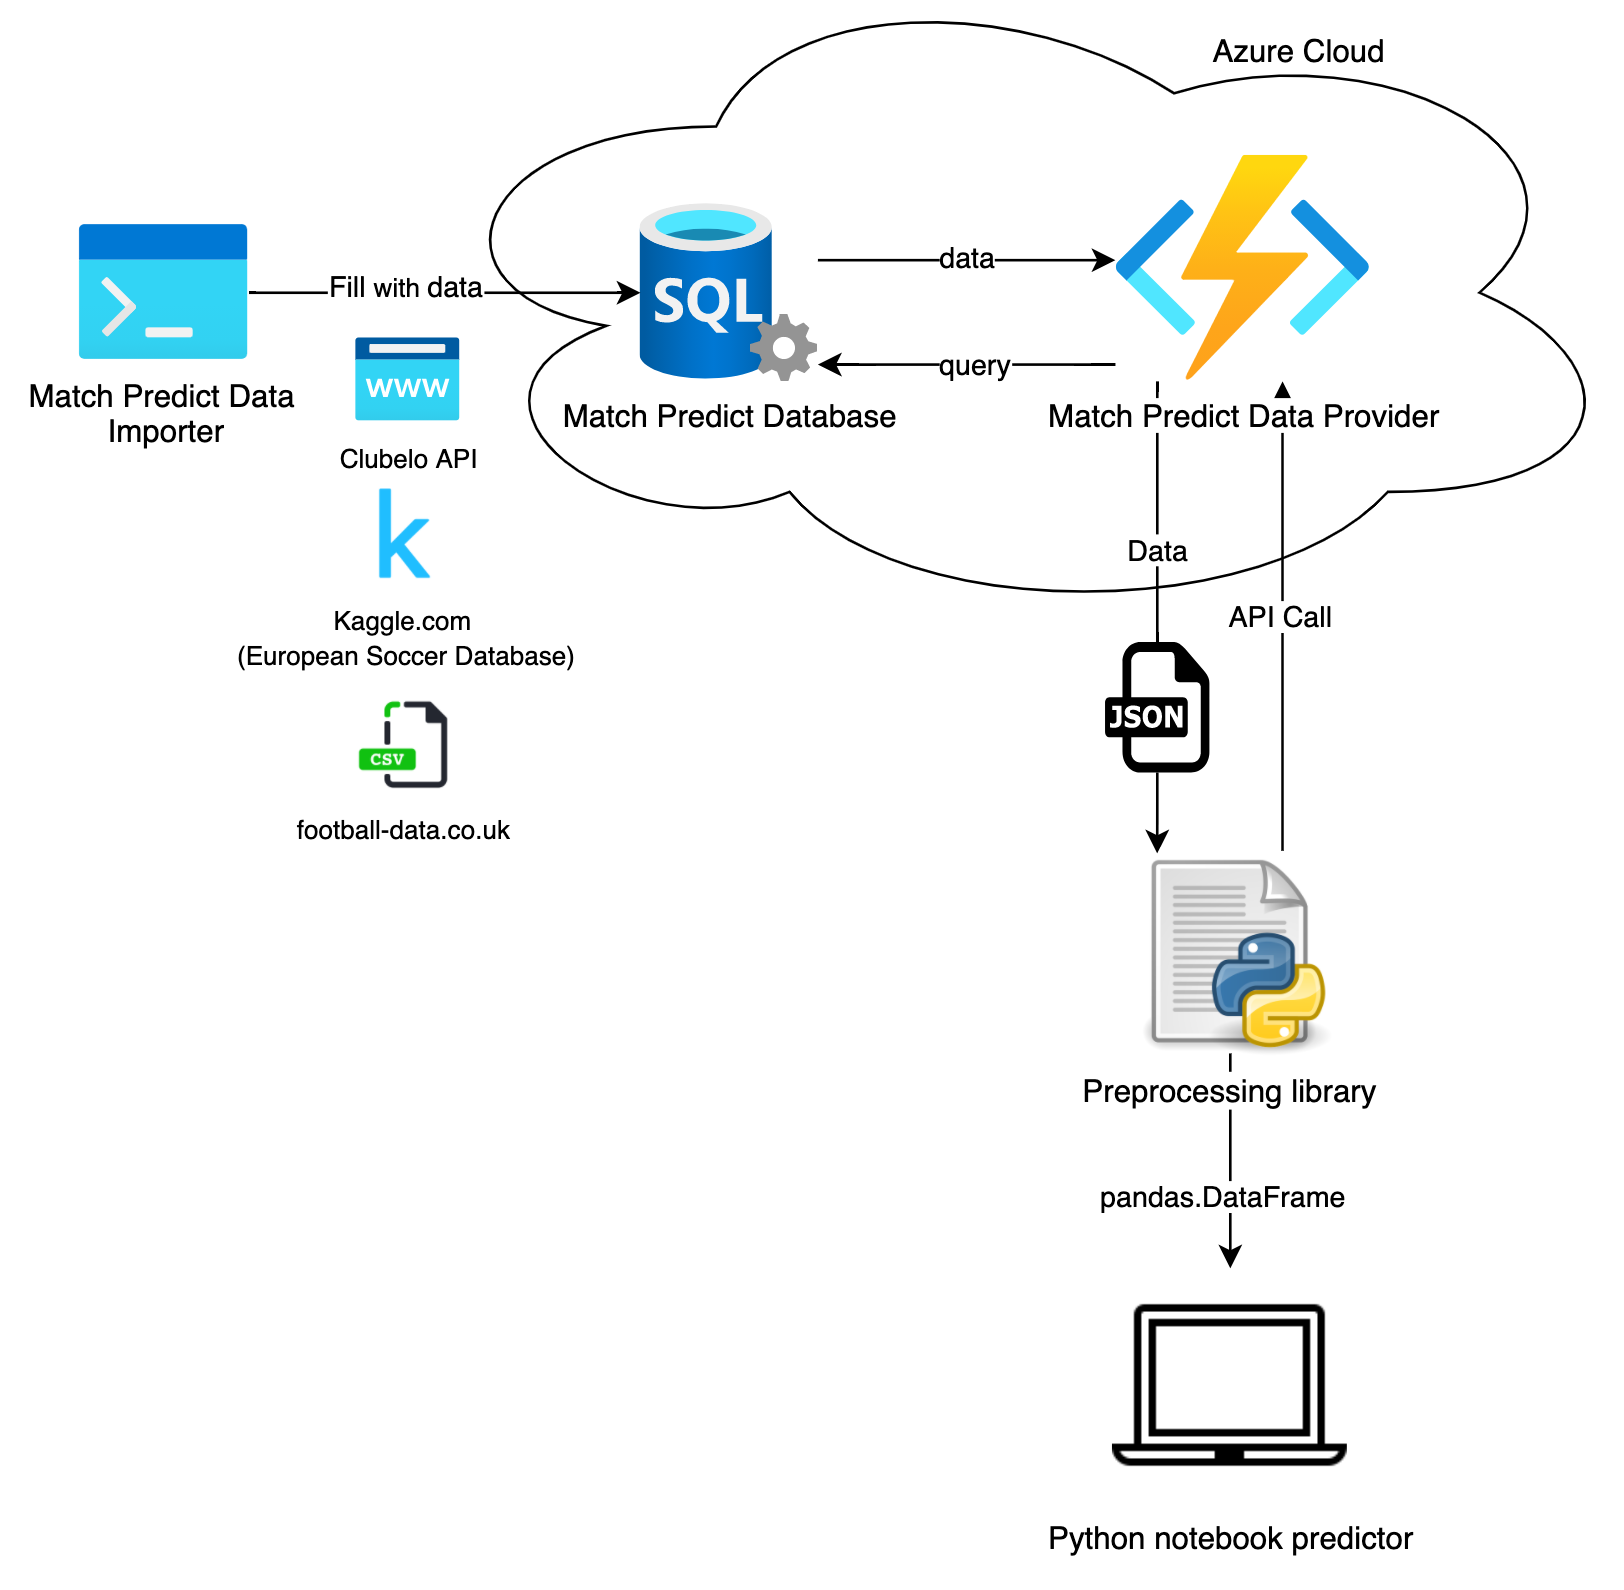
\includegraphics[width=\textwidth]{figures/MatchPredictorArchitecture.png}
        \caption{Architektura systemu Soccer Match Predictor}\label{fig:arch1}
    \end{figure}
    \newpage

\noindent Pierwszym komponentem jest \textbf{Match Predict Data Importer}, dalej nazywany MPDI. Jest to aplikacja konsolowa napisana w języku C\#, której zadaniem jest import danych z różnych źródeł do docelowej bazy danych widocznej jako \textbf{Match Predict Database} na schemacie.

Baza jest przechowywanym na chmurze Azure komponentem Microsoft SQL Server, w której przechowywane są wszelkie dane wykorzystywane dalej w systemie. Schemat bazy danych jest przedstawiony w sekcji \ref{database_schema}.

Match Predict Data Provider (dalej zwany MPDP) służy w produkcie jako WebAPI, które przesyła dane w formacie JSON. Dane pochodzą z bazy Match Predict Database i są odpowiednio agregowane. Komponent ten to aplikacja Azure Function napisana w języku C\#, która znajduje się na chmurze Azure.\\



Kolejnym komponentem w systemie widocznym na schemacie jako \textbf{Preprocessing library} jest biblioteka służąca do pobierania danych i ich wstępnego przetwarzania wraz z tworzeniem zbioru cech. Jest to moduł napisany w języku Python, który może być wykorzystany w dowolnej aplikacji napisanej w tym języku. Komunikuje się on z opisaną wyżej bazą danych przy pomocy udostępnionego przez nią interfejsu WebAPI i otrzymuje od niego dane w formacie JSON, natomiast korzystającym z niego klientom przekazuje wygodne do operowania dane w formacie pandas.DataFrame. 

Uniwersalność tego modułu polega na tym, że całkowicie chowa on szczegóły implementacji swoich operacji pobierania danych z bazy, przetwarzania ich i tworzenia cech i udostępnia jedynie metody pozwalające na pobranie danych dla konkretnych sezonów i/lub konkretnych drużyn. Dzięki temu klient korzystający z tego modułu jest niezależny od wszelkich zmian strukturalnych w bazie danych czy interfejsie służącym do komunikacji z nią.\\


Ostatnim elementem jest widoczny na schemacie \textbf{Python notebook predictor}, który służy jako środowisko testowe do porównywania różnego rodzaju algorytmów stosując różne podejścia i techniki. Jest to aplikacja stworzona w \textit{Jupter Notebook}, czyli rozbudowanym narzędziu uruchamianym w przeglądarce internetowej pozwalającym na m.in. separowanie poszczególnych części kodu i uruchamianie ich niezależnie od siebie. Pozwala to na przykład na jednorazowe pobranie danych na samym początku i wielokrotne użycie ich w późniejszych eksperymentach.

Środowisko to jest klientem opisanego wyżej modułu do wstępnego przetwarzania danych i korzysta z niego do pobierania przetworzonych danych. 


\section{Schemat bazy danych}
\label{database_schema}
\section{Opis web API}
\section{Środowisko użytkownika docelowego}
\section{Ew. dodatkowe narzędzia analizy danych}